%
% File acl2017.tex
%
%% Based on the style files for ACL-2015, with some improvements
%%  taken from the NAACL-2016 style
%% Based on the style files for ACL-2014, which were, in turn,
%% based on ACL-2013, ACL-2012, ACL-2011, ACL-2010, ACL-IJCNLP-2009,
%% EACL-2009, IJCNLP-2008...
%% Based on the style files for EACL 2006 by 
%%e.agirre@ehu.es or Sergi.Balari@uab.es
%% and that of ACL 08 by Joakim Nivre and Noah Smith

\documentclass[11pt,a4paper]{article}
\usepackage[utf8]{inputenc}
\usepackage[hyperref]{acl2017}
\usepackage{times}
\usepackage{latexsym}
\usepackage{amsmath}
\usepackage{amsfonts}
\usepackage{algorithm}
\usepackage{xcolor}
\usepackage{algpseudocode}
\usepackage{graphicx}
\usepackage{footnote}
\usepackage{footmisc}
\usepackage{footnotebackref}
\newcommand*\Let[2]{\State #1 $\gets$ #2}  
\usepackage{url}
\usepackage{listings}
\usepackage{CJKutf8}
\usepackage{qtree}
% \usepackage{pdfpages}

\usepackage{tikz}
\usetikzlibrary{arrows,automata}
\usepackage{subcaption}
\definecolor{fijecomment}{RGB}{64,224,208}
%\aclfinalcopy % Uncomment this line for the final submission
%\def\aclpaperid{***} %  Enter the acl Paper ID here

%\setlength\titlebox{5cm}
% You can expand the titlebox if you need extra space
% to show all the authors. Please do not make the titlebox
% smaller than 5cm (the original size); we will check this
% in the camera-ready version and ask you to change it back.

\newcommand\BibTeX{B{\sc ib}\TeX}

\title{Machine Translation with a Latent Variable \\ Conditional Random Field}% \\ NLP2 project 2}}

\author{Tim van Elsloo \\
 10590315\\\And
  Fije van Overeem \\
  10373535 \\\And 
  Daan van Stigt \\
  10255141    }

\date{}

\begin{document}
\maketitle
\begin{abstract}
A probabilistic model for hierarchical machine translation is implemented: a Conditional Random Field (CRF) with latent Inversion Transduction Grammar (ITG) derivations, mapping from a source sentence $x$ to a target sentence $y$. Training on 40k Chinese-English sentence pairs yields a BLEU score of 4.04 on the training set and 0.00 on test set. Even though the BLEU scores are low, the model's learning ability is impressive given the large and complex hypothesis-space generated by the ITG.
\end{abstract}

\section{Introduction}

This paper reports on a probabilistic model for hierarchical machine translation, partly inspired by the model of Blunsom et al \cite{blunsom2008discriminative}. We have seen that IBM Model 1 and 2 can be used to train an alignment model for words with a source language and a target. One of IBM1's problems is that it cannot train and infer word order for the translation of a sentence.

Our goal is to perform the full translation task: translating a source sentence $x$ into a target sentence $y$. To this end, we firsts construct a latent Inversion Transduction Grammar (ITG) tree mapping between $x$ and possible translations $y$. An ITG is a compact way to represent the large number of canditate translations $y$ for $x$ created by translating, deleting, inserting and permuting the words in $x$ \cite{wu97}. For the lexical operations we use a constrained vocabulary given by the top translation under trained IBM1 word-alignments. We then fit a Latent-Variable Conditional Random Field (LV-CRF) to observed translation-pairs $(x,y)$ using a stochastic optimization procedure on a weights vector vector $w$. 

The paper is structured as follows. In Section 2 we describe our model in detail: the ITG and the LV-CRF. We describe how we can fit this model to observations using stochastic optimization, and how the required quantities for this can be obtained efficiently using dynamic programming in Section 3. In Section 4 we describe how we can use the trained model to perform inference: choosing an optimal translation $y$ for a new source sentence $x$. Then in Section 5 we describe the results of an experiment we performed with the model on a Chinese to English translation task, and in Sections 6 and 7 we describe and discuss these results.

\section{Model}

In this section we describe our model: a LV-CRF on top of an ITG. First we describe the ITG as an example of bitext parsing.

\subsection{Bitext parsing}

The ITG in our model is formulated as the constrained Synchronous Context Free Grammar (SCFG) given by the rules in figure \ref{fig:scfg}. This grammar is fit for the task of bitext-parsing: simultaneously parsing two sentences $x$ and $y$. 

The rules in figure \ref{fig:scfg} specify how productions from the source CFG that parses $x$ are to be transformed to obtain productions in a target CFG that parses $y$. Each rule in the source CFG of the form $\text{S} \to \text{X}$ is copied to the target CFG. Then for each rule $\text{X} \to \text{X}_1 \text{X}_2$ in the source CFG both a \textit{monotone} copy $\text{X} \to [\text{X}_1 \text{X}_2]$ and an \textit{inverted} copy $\text{X} \to \langle\text{X}_2 \text{X}_1\rangle$ are added to the target CFG. Then lastly, for each lexical rule $\text{X} \to \alpha$ in the source CFG, a \textit{translation} given by $\text{X} \to \alpha/\beta$, an $insertion$ given by $\text{X} \to \epsilon/\beta$, and a $deletion$ given by $\text{X} \to \alpha/\epsilon$ are introduced to the target CFG.

\begin{figure}[H]
\center
\begin{align*}
    \text{S} &\to \text{X} \\
    \text{X} &\to [\text{X X}] \\
    \text{X} &\to \langle\text{X X}\rangle \\
    \text{X} &\to \alpha/\beta \quad \text{where } \alpha\in \Sigma_{\alpha} \text{ and }  \beta\in \Delta_{\beta} \\
    \text{X} &\to \epsilon/\beta \quad \text{where } \beta\in \Delta_{\beta} \\
    \text{X} &\to \alpha/\epsilon \quad \text{where } \alpha\in \Sigma_{\alpha}
\end{align*}
\caption{A constrained SCFG over constrained source vocabulary $\Sigma_{\alpha}$ and target vocabulary $\Delta_{\beta}$, where $\epsilon$ denotes the empty string.}
\label{fig:scfg}
\end{figure}
Given the constrained SCFG, we can generate the following sets:
\begin{align*}
    \mathcal{D}(x,y) &= \{d: \text{yield}_{\Sigma}(d)= x \text{ and } \text{yield}_{\Delta}(d)= y\}  \\
    \mathcal{D}_n(x) &= \{d: \text{yield}_{\Sigma}(d)= x \text{ and } |\text{yield}_{\Sigma}(d)|\leq n\},
\end{align*}
where $\mathcal{D}_{n}(x)$ is the set of derivations compatible with $x$ constrained to yield sentences no longer than $n$ words, and $\mathcal{D}(x,y)$ is the set of derivations compatible with both $x$ and its translation $y$. These sets will form the basis of the training.

These sets are obtained by parsing the sentences $x$, $y$, and $x$ and $y$ together. This process can be viewed as intersecting the language generated by the (S)CFG with the language generated by a Finite State Automaton (FSA) \cite{BarHillel61}, representing in this case respectively $x$ and $y$. We describe the full procedure below. From now on we refer to the sets $\mathcal{D}_{n}(x)$ and $\mathcal{D}(x,y)$ as \textit{forests}: sets of derivation trees.

\subsubsection{Obtaining $\mathcal{D}_{n}(x)$ and $\mathcal{D}(x,y)$}
\label{sec:fsa}
Consider the source sentence $x=$\textit{ des chiens noirs} paired with the target sentence $y=$\textit{ black dogs}. These sentences can be represented as a simple linear-chain FSA with the transitions between states given by the sentence's words in order. Figure \ref{fig:source-fsa} shows the resulting source FSA and figure \ref{fig:target-fsa} the target FSA.
\begin{figure}[H]
    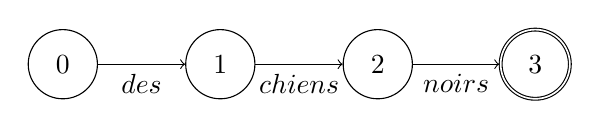
\begin{tikzpicture}[node distance=2.0cm]
        \node[state] (0) {0};
        \node[state, right of=0] (1) {1};
        \node[state, right of=1] (2) {2};
        \node[accepting, state, right of=2] (3) {3};
        
        \draw (0) edge[->] node[below] {$des$} (1);
        \draw (1) edge[->] node[below] {$chiens$} (2);
        \draw (2) edge[->] node[below] {$noirs$} (3);
    \end{tikzpicture}
    \caption{Source FSA. Finite states are denoted with double circles.}
    \label{fig:source-fsa}
\end{figure}
\begin{figure}[H]
\center
    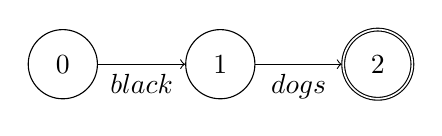
\begin{tikzpicture}[node distance=2.0cm]
        \node[state] (0) {0};
        \node[state, right of=0] (1) {1};
        % \node[state, right of=1] (2) {2};
        \node[accepting, state, right of=1] (2) {2};
        
        \draw (0) edge[->] node[below] {$black$} (1);
        \draw (1) edge[->] node[below] {$dogs$} (2);
        % \draw (2) edge[->] node[below] {dog} (3);
    \end{tikzpicture}
    \caption{Target FSA.}
    \label{fig:target-fsa}
\end{figure}
Using an Earley parser \cite{earley}, the simple source CFG given in figure \ref{fig:source-cfg}, and the source FSA, we parse the source sentence $x$ to yield the source forest. A forest is represented as a set of items: rules where symbols are annotated with spans, representing the fragment of the sentence that is recognized to be under that symbol. A fragment of the forest is shown in figure \ref{fig:source-forest}.
\begin{figure}
\center
\begin{align*}
    \text{S} &\to \text{X} \\
    \text{X} &\to \text{ X X } \\
    \text{X} &\to \alpha \quad\text{for } \alpha\in \Sigma
\end{align*}
\caption{The source CFG.}
\label{fig:source-cfg}
\center
\begin{align*}
    \text{S}_{0:3} &\to \text{X}_{0:3} \\
    \text{X}_{0:3} &\to \text{X}_{0:1} \text{X}_{1:3} \\
    \text{X}_{0:1} &\to des_{0:1}  \\
    \text{X}_{1:3} &\to \text{X}_{1:2} \text{X}_{2:3} \\
    \text{X}_{1:2} &\to chiens_{1:2} \\
    \text{X}_{2:3} &\to noirs_{2:3}
\end{align*}
\caption{Parse forest for $x =$\textit{ des chiens noirs}.}
\label{fig:source-forest}
\end{figure}
In order for our probabilistic model to be well-defined, we need to make sure that $\mathcal{D}(x)$ is a finite set. To achieve this we intersect the language with a special insertion-constrained-FSA pictured in \ref{fig:eps-fsa}. Note that the wildcard symbol (*) may be reduced to any non-terminal (word) in the target language. This way we will insert at most $n$ words into the target-yield. We call the resulting forest $\mathcal{D}'_n(x)$. 
\begin{figure}[H]
\center
    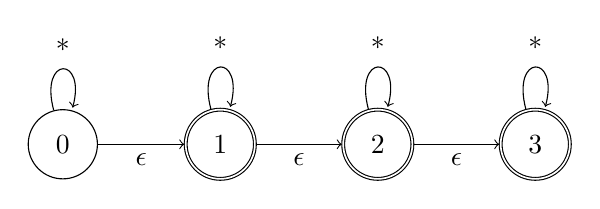
\begin{tikzpicture}[node distance=2.0cm]
        \node[state] (0) {0};
        \node[accepting, state, right of=0] (1) {1};
        \node[accepting, state, right of=1] (2) {2};
        \node[accepting, state, right of=2] (3) {3};
        
        \draw (0) edge[->] node[below] {$\epsilon$} (1);
        \draw (0) edge[loop above] node[above] {*} (0);
        \draw (1) edge[->] node[below] {$\epsilon$} (2);
        \draw (1) edge[loop above] node[above] {*} (1);
        \draw (2) edge[->] node[below] {$\epsilon$} (3);
        \draw (2) edge[loop above] node[above] {*} (2);
        \draw (3) edge[loop above] node[above] {*} (3);
    \end{tikzpicture}
    \caption{Insertion constrained FSA with $n=3$.}
    \label{fig:eps-fsa}
\end{figure}

From this forest we obtain $\mathcal{D}_n(x)$ by projecting the items (annotated rules) in $\mathcal{D}'_n(x)$ using the ITG rules given in figure \ref{fig:scfg}.The translations, insertions, and deletions are constrained for the forests to remain manageable. For this we use a lexicon with only top-$k$ translations under some translation distribution $P$. In our case this distribution is given by pre-trained IBM1 alignment probabilities and provides the translation probabilities $P(\beta | \alpha)$, insertion probabilities $P(\beta | \epsilon)$ and deletion probabilities $P(\epsilon | \beta)$. An example for Chinese-English is given in table \ref{table:lexicon}, which is from the lexicon that we use in the experiments.
\begin{figure}[H]
\centering
\begin{CJK}{UTF8}{gbsn}
\begin{tabular}{c|c|c|c|c}
$\alpha$  & $\beta$ & $P(\beta | \alpha)$ & $P(\beta | \epsilon)$ & $P(\epsilon | \beta)$ \\ \hline
折 & give & 2.25e-10 & 1.38e-20 & 9.88e-17 \\
\end{tabular}
\end{CJK}
\caption{Example lexicon.}
\label{table:lexicon}
\end{figure}
By this procedure we have obtained the set $\mathcal{D}_n(x)$: all possible translations generated by the ITG projection rules from the forest compatible with the source sentence $x$ with at most $n$ $\epsilon$-insertions.

% \subsubsection{Resulting forest $\mathcal{D}(x,y)$}%Translation Observation during Training}

% During training the correct translation $y$, represented as the FSA in \ref{fig:target-fsa}, is known.
% Remember that we used the source CFG and the source FSA to create a forest: we now use the target CFG and the target FSA to create a forest for the target sentence. Note that the target CFG is the source forest projected to the target lexicon. The resulting forest contains all derivations that are compatible with source sentence $x$ and target sentence $y$. We call this set $\mathcal{D}(x, y)$.

Lastly, we can obtain the set $\matcal{D}(x,y)$, the set of derivations that in addition to $x$ also produce the target observation $y$. Again, we do that by intersecting a CFG with an FSA. This time these are the projected forests $D_n(x)$ with the FSA that represents $y$ given in figure \ref{fig:target-fsa}.
\begin{figure}
\begin{subfigure}{\linewidth}
        \Tree[.S$_{0:3,0:2}$ [.X$_{0:3,0:2}$ [.X$_{0:1,0:0}$ [.$des/\epsilon$ ]] [.X$_{1:3,0:2}$ [.X$_{1:2,2:3}$ [.$chiens/dogs$ ]] [.X$_{2:3,1:2}$ [.$noirs/black$ ]]]]] \\
\caption{derivation $d$ as tree.}
\end{subfigure}
\begin{subfigure}{\linewidth}
\begin{align*}
    \text{S}_{0:3,0:2} &\to \text{X}_{0:3,0:2} \\
    \text{X}_{0:3,0:2} &\to \text{X}_{0:1,0:0} \text{ X}_{1:3,0:2} \\
    \text{X}_{1:3,0:2} &\to \text{X}_{1:2,2:3} \text{ X}_{2:3,1:2} \\
    \text{X}_{0:1,0:0} &\to des/\epsilon \\
    \text{X}_{1:2,2:3} &\to chiens/dog \\
    \text{X}_{2:3,1:2} &\to noirs/black
\end{align*}
\caption{Derivation $d$ as list of items (annotated rules).}
\end{subfigure}
\caption{Example derivation $d$ from the set $\mathcal{D}(x,y)$. For ease of comprehension we've omitted the spans on the lexical items.}
\end{figure}

% The possible translations for each word are completed with probability for an $\epsilon$ translation: the option that the word translates to nothing. 
Note that in order for the set $\mathcal{D}(x,y)$ to be non-empty, the target sentence $y$ should be in the yield of $\mathcal{D}_n(x)$. This is determined both the number of insertions $n$ as well as the number of translations $k$ we allow. As we will see, for small $n$ and $k$, $\mathcal{D}(x,y)$ will often be empty. Table \ref{table:experiment} shows the results of a small experiment on the effect of the number of translations on the number of empty forests $\mathcal{D}(x,y)$ derived from a set of 300 forests $\mathcal{D}_n(x)$.
% It intuitively means that the probability to be able to translate to a reference sentence increases, since the amount of possible target sentences is bigger.
    \begin{table}[]
        \centering
        \begin{tabular}{c|c | c}
            $\mathcal{D}_n(x)$ & $k$ & Non-empty $\mathcal{D}(x,y)$ \\ \hline
            300 & 3 & 30 \\
            300 & 6 & 52
        \end{tabular}
        \caption{Small experiment to illustrate the effect of amount of translations on resulting reference forests}
        \label{table:experiment}
    \end{table}



\subsection{LV-CRF}

In this section we describe the Latent Variable Conditional Random Field (LV-CRF) that we use to probabilistically model the translation process that is given by the deterministic ITG.

The model is shown in graphical form in figure \ref{fig:crf}. Here $x$ and $y$ are the source sentence and target sentence respectively, $n$ is the maximal number of insertions, $d$ is the latent ITG tree, and $w$ is a parameter-vector that we will use to fit the model to the training data. The plate indicates that we assume independence over sentences $s$ in the corpus $S$. Note that $x$ and $n$ are fully observed, but that $y$ is partially observed: only during training time do we have access to $y$; during prediction it is not. 

The LV-CRF model is a Random Field due to presence of undirected edges; it is Latent Variable, because of the latent derivations $d$; and lastly it is Conditional because we not to model the probability of $x$: the source sentence is fully observed at all times. Hence the name.

\begin{figure}[H]
\center
    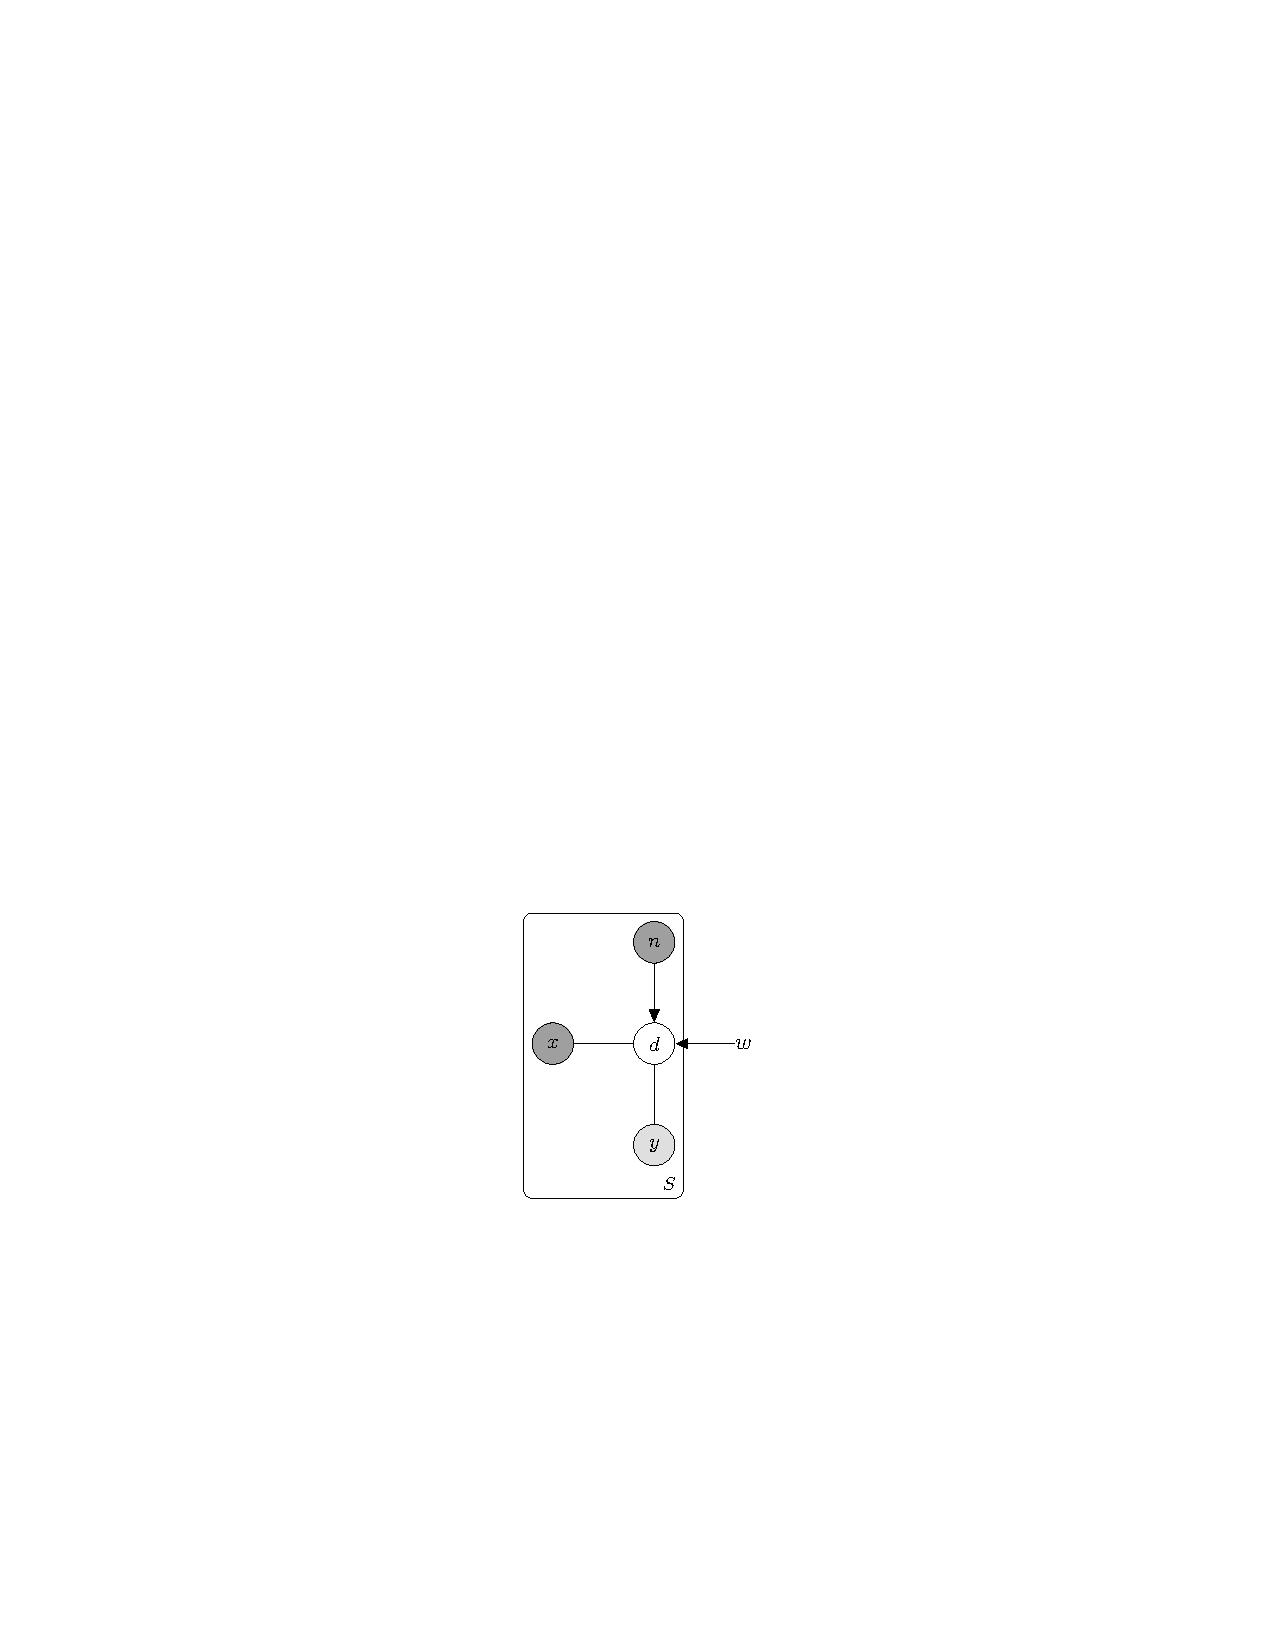
\includegraphics[scale=0.9]{images/graphical-model.pdf}
    \caption{Conditional random field for translation with latent ITG trees $d$.}
    \label{fig:crf}
\end{figure}
For each sentence $s$ the maximal clique in the model is given by $C=\{y, d, x\}$. The variables $y,d,x$ are thus correlated, without specifying a causal relation. Our choice is to define the factor
\begin{align*}
f(y,d,x) = \exp(w^{\top}\Phi(y,d,x)) 
\end{align*}
where $\w \in \mathbb{R}^d$ is a parameter vector and $\Phi: \matcal{D} \to \mathbb{R}^d$ a deterministic feature function mapping a parse forest to $\mathbb{R}^d$.

The latent derivations $d$ are the parse forest $\mathcal{D}_n(x)$
and $\mathcal{D}(x,y)$ introduced above. We can picture these forests as hypergraphs, where the hyper-edges correspond to rules: a rule of the form $\text{X}_{1:3}\to\text{X}_{1:2}\text{X}_{2:3}$ corresponds to a directed hyper edge from the nodes $\text{X}_{1:2}\text{X}_{2:3}$ to the node $\text{X}_{1:3}$. An illustration of this hypergraph interpretation of a parse forest is given in figure \ref{fig:decoding}. One nice feature that these hypergraphs have is that the factor $\Phi(y,d,x)$ factors along the hyper-edges. Let us denote such an hyper-edge as $r_{s,t}$, which we read as a rule decorated with source span $s$ and target span $t$. Then we can factor $f$ along the edges as
\begin{align*}
    f(y,d,x) 
        &= \prod_{r_{s,t}\in d}f'(r,s,t,x,n) \\
        &= \prod_{r_{s,t}\in d}\exp(w^{\top}\phi(r,s,t,x,n) \\
        &= \exp\Big(\sum_{r_{s,t}\in d}w^{\top}\phi(r,s,t,x,n)\Big),
\end{align*}
where $\phi$ is now a $local$ feature function mapping rules $r_{s,t}$ to $\mathbb{R}^d$.
\begin{figure}[H]
    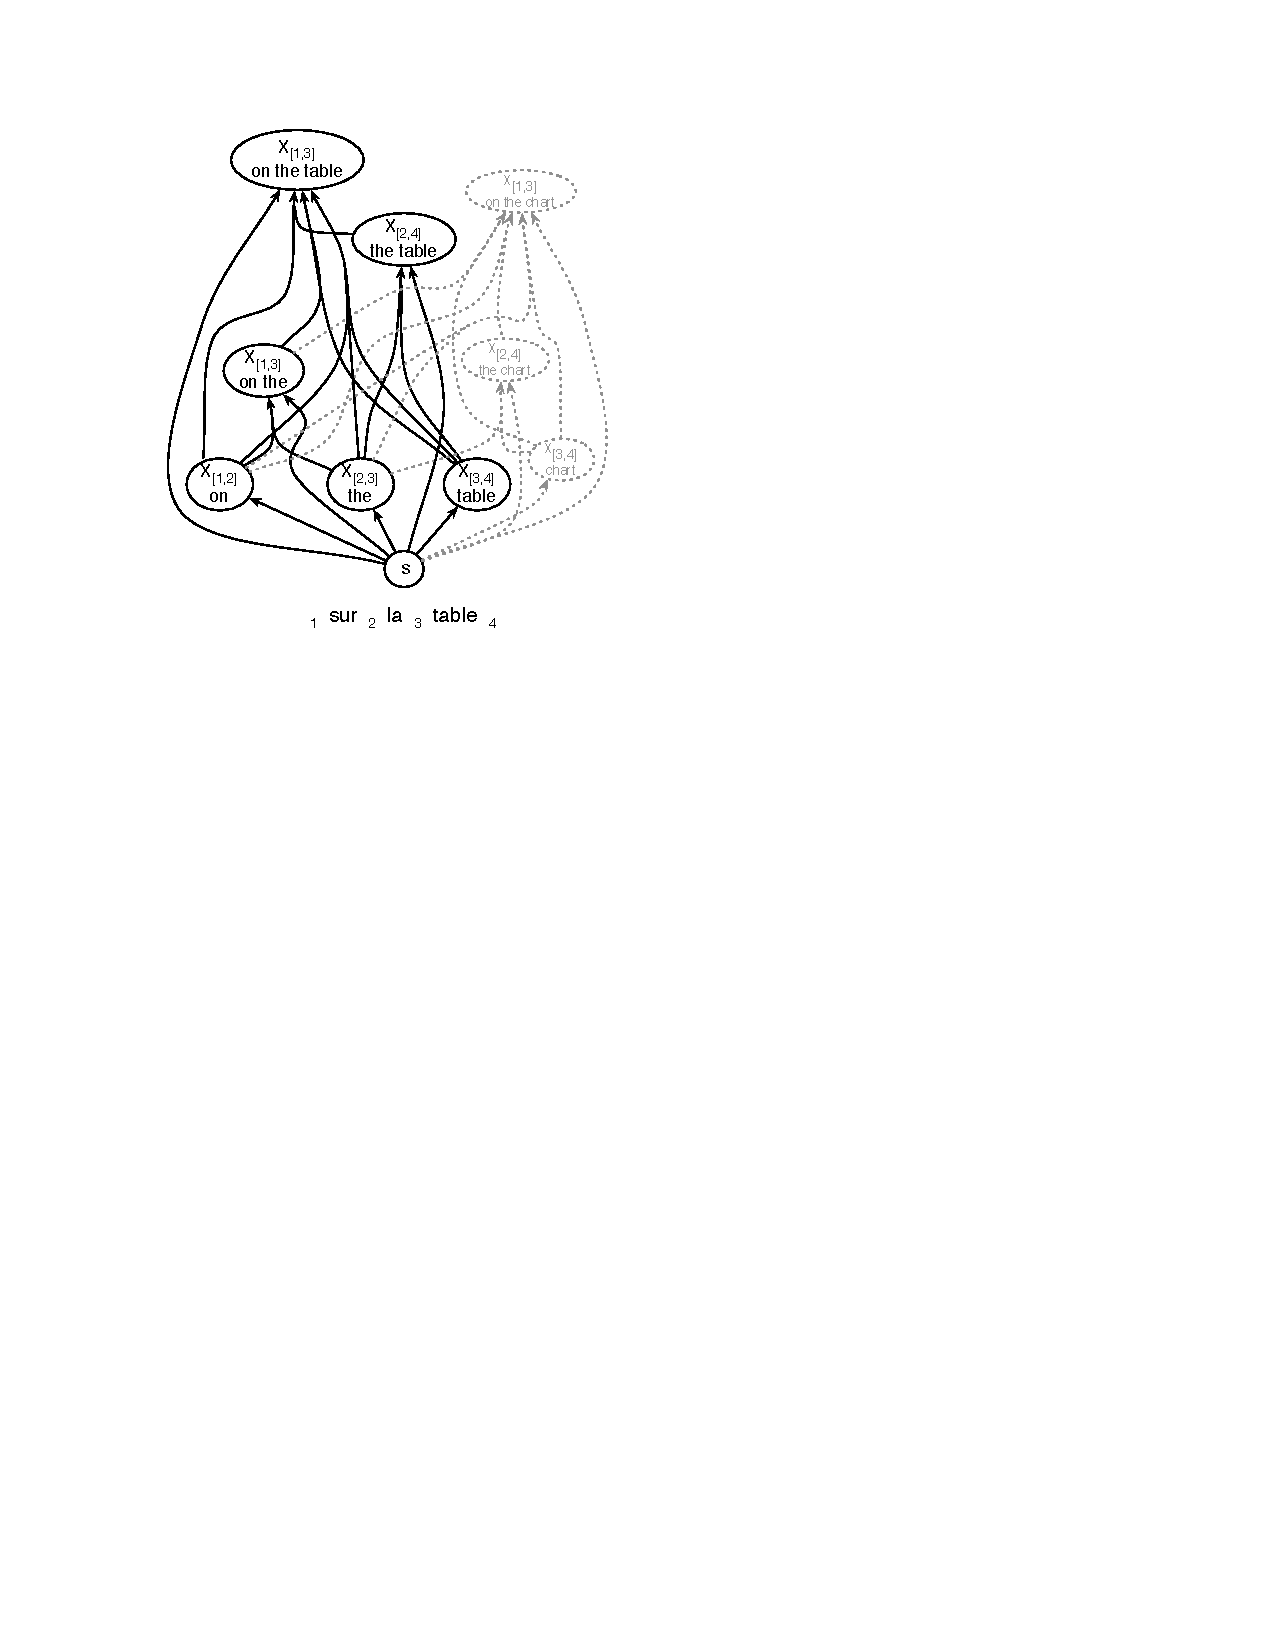
\includegraphics[scale=0.9]{images/CRF.pdf}
    \caption{Hypergraph representation of a section of a parse forest, taken from \cite{blunsom2008discriminative}. The figure shows a number of possible derivations---some of which are shown transparently---represented as paths along the hyper-edges from root to lexical leafs. Note that we are using a slightly different notation convention, which should not obscure the general message.}
    \label{fig:decoding}
\end{figure}

\subsection{Likelihood}
\label{sec:model}

Given the LV-CRF above, we can now specify the joint probability of a sentence $y$ and a derivation $d$ given an source sentence $x$. It is given by the equation
\begin{align*}
\label{eq:likelihood}
P(y,d|x) 
    &= \frac{\exp(w^\top \Phi(y, d, x))}{\sum_{d' \in \mathcal D_n(x)} \exp(w^\top \Phi(y', d', x))}\\
    &= \frac{\exp(w^\top \Phi(y, d, x))}{Z_n(x)} \\
    &= \frac{\exp \left( \sum_{r_{s,t} \in d} w^\top \phi(r, s, t, x, n) \right)}{Z_n(x)}.
\end{align*}
Here $\mathcal{D}_n(x)$ is the support for the joint distribution $P(Y, D|X=x, N=n)$ and $\mathcal{D}(x, y)$ is the support for the posterior distribution $P(D|X=x, Y=y, N=n)$.

The likelihood of an observation $y$ is obtained by marginalizing out the derivations $d$:


\begin{align}
P(y | x, w) 
    &= \sum_{d \in \mathcal{D}_n(x)} P(y, d | x, w) \nonumber  \\
    &= \frac{\sum_{d \in \mathcal D(x, y)} \exp(w^\top \Phi(y, d, x, n))}{Z_n(x)} \nonumber \\
\label{eq:log-likelihood2}
    &= \frac{Z(x, y)}{Z_n(x)}
\end{align}

\subsection{Features}

The local feature function $\phi$ featurizes the edges of the parse forest. This function is hand-crafted and classifies the edges in one of the categories
\begin{itemize}
    \item Translation  
    \item Deletion
    \item Monotone/Inverted
    \item Unary/Binary
    \item Skip bi-gram
\end{itemize}
First it counts the number of spans on the right hand side. Because the grammar is in CNF, this is always either 1 (unary rule) or 2 (binary rule). For example, this feature would be unary for the first and third rule, and binary for the second rule in fig. \ref{fig:source-forest}. Another feature could be whether or not a rule reverses its spans.
To understand why these features can be used to train translation algorithms intuitively, take an example for deletion: When translating the words `ne .. pas' from French to English, the algorithm learns that deletion often occurs with this context, which leads to a higher probability of the translation to `not', where one of the French words is in fact deleted.


\section{Training}

In this section we describe the method by which we fit the LV-CRF model using the weights $w$ to training instances.

\subsection{Stochastic Optimization}

The log-likelihood of an observation $(x,y)$, given by
\begin{align*}
\label{eq:log-likelihood}
\mathcal{L}(w|x,y,n) &= \log P(y|x, n) \\
    &= \log Z(x,y) - \log Z_n(x).
\end{align*}
Following the maximum likelihood principle we maximize the likelihood of the observation $(x,y)$ under $\log P(y|x, n)$. We do this by optimizing the above expression with respect to $w$. For this we use Stochastic Gradient Descent (SGD). Taking the gradient with respect to $w$ of $\mathcal{L}$ we get that
\begin{align*}
\nabla_w\mathcal{L}(w|x,y,n) 
    &= \mathbb{E}_{P_{D|x,y,n,w}}[\phi(X,Y,D)] \\
    &\quad- \mathbb{E}_{P_{Y, D|x,n,w}}[\phi(X,Y,D)].
\end{align*}
The update rule at step $t+1$ for the stochastic optimization procedure is then given by
\begin{align*}
    w^{(t+1)} = w^{(t)} + \delta^{(t)}\nabla_{w^{(t)}}\mathcal{L}(w^{(t)}|x,y,n),
\end{align*}
where $\delta^{(t)}$ is the learning rate at step $t$. We use an adaptive scheme for the learning rate following \cite{Bottou12}, where we let the learning rate decay as an inverse exponential of the number of parameter-updates. We define the learning $\delta^{(t)}$ at parameter-update $t$ to be
\begin{align*}
\delta^{(t)} = \delta^{(0)} (1 + \gamma\delta^{(0)} t)^{-1}
\end{align*}
where $\delta^{(0)}$ is the initial learning rate at $t=0$ and $\gamma$ and additional hyperparameter to determined. See figure  \ref{fig:learning-rates} for the effect of different values of $\gamma$.

\begin{figure}[H]
    \centering
    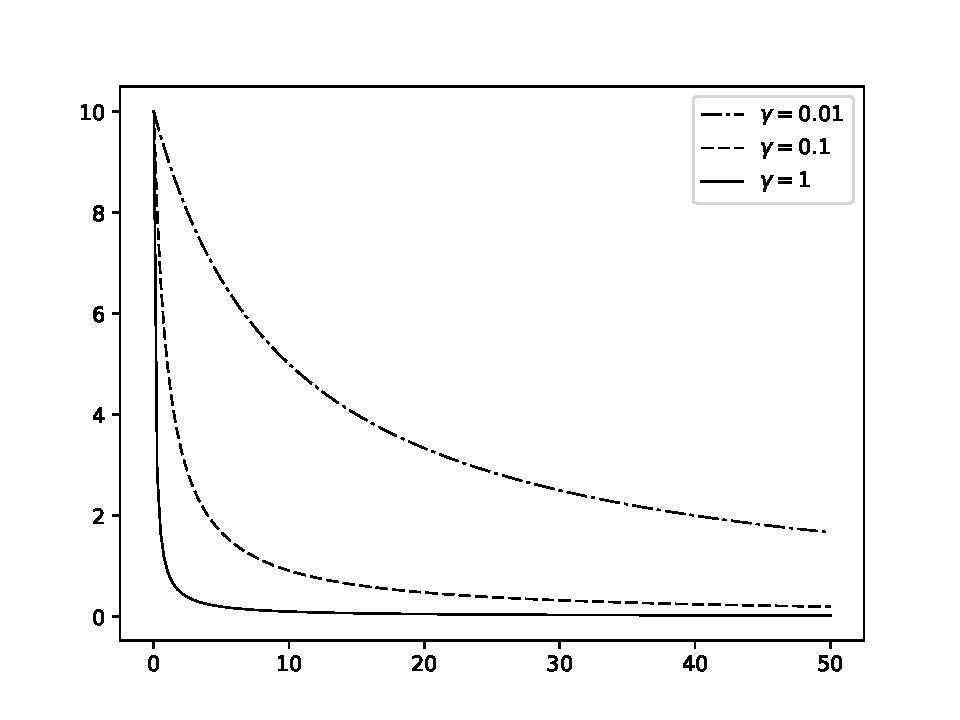
\includegraphics[width=\linewidth]{images/learning-rates.pdf}
    \caption{Effect of $\gamma$ on the decay of the learning rate for a starting rate $\delta^{(0)} = 10$.}
    \label{fig:learning-rates}
\end{figure}



\subsection{Regularization}

The update formula with $L_2$ regularization term $L_2$ is given by
\begin{align*}
\nabla_w\mathcal{L}(w|x,y,n) 
    &=\mathbb{E}_{P_{D|x,y,n,w}}[\phi(X,Y,D)] \\
    &\quad-\mathbb{E}_{P_{Y, D|x,n,w}}[\phi(X,Y,D)] \\
    &\quad- 2\lambda w.
\end{align*}
where $\lambda$ is a hyperparameter the value of which is to be  determined.


\subsection{Efficiently computing log-normalizer}

In order to compute the likelihood and subsequently perform stochastic optimization on $w$, we need to be able to efficiently compute the log-normalizers $\log Z(x, y)$, which explains the translation pair $x$ and $y$, and $\log Z_n(x)$, which marginalizes over all derivations of $x$. 

Since our model is represented as an acyclic hypergraph (sec. \ref{sec:model}), there is an efficient algorithm for this called the inside-outside algorithm \cite{Lari90}, which is a hypergraph generalization of the forward-backward algorithm. The inside values are computed recursively by the following equations:
\begin{equation*}
    I(v) = \begin{cases}
        1 \qquad\text{if BS(v) is empty} \\
        \sum\limits_{e \in \textrm{BS}(v)} w(e) \prod\limits_{u \in \textrm{tail}(e)} I(u)
    \end{cases},
\end{equation*}
where $w(e)$ is the weight function that assigns a score to edge $e$ based on its features (sec. \ref{sec:model}). The inside value at the root of the forest then gives the log-normaliser $\log Z$ of the forest.

In order to efficiently compute the expected feature vectors, which we need for the stochastic optimizer's update-rule, we need additionally need $outside$ values of a node \cite{Li09}. These are given by the following equations, for which we require the inside values first:
\begin{equation*}
    O(v) = \begin{cases}
        1 \qquad\text{if FS(v) is empty} \\
        \sum\limits_{e \in \textrm{FS}(v)} w(e) O(\textrm{head}(e)) \prod\limits_{s \in \textrm{tail}(e) \backslash \{ v \}} I(s)
    \end{cases},
\end{equation*}
Both the inside and the outside recursions can be computed by iteratively visiting the nodes in the hypergraph in topologically-sorted order.\footnote{ A topological ordering of a directed graph is a linear ordering of its vertices such that for every directed edge $(u,v)$ from vertex $u$ to vertex $v$, $u$ comes before $v$ in the ordering.}.

\section{Inference}
Once we have obtained a trained weight vector $w$ we would like to predict the best translation $y$ for a source sentence $x$. In this section we describe how this can be done efficiently (but approximately).

\subsection{Viterbi decoding}

In order to compute translations, we use the Viterbi algorithm to find the derivation in the target language that maximizes the probability. Viterbi is an efficient dynamic programming algorithm to find the optimal path in a hypergraph (fig. \ref{fig:decoding}). However, if we were to define our decoding scheme with eq. \ref{eq:viterbi-intractable}, the solution would be intractable because we marginalize over $\mathcal{Y}_n(x)$: all latent derivations of $x$ in the target language.

\begin{equation}
    \label{eq:viterbi-intractable}
    y^\star = \operatornamewithlimits{arg max}_{y \in \mathcal{Y}_n(x)} P(y, d | x)
\end{equation}

Instead, we use an approximation of the Viterbi decoding. This approximation does not necessarily have to equal the optimal path, but it is tractable.

\begin{equation}
    y^\star = \textrm{yield}_\Delta \left\{ \operatornamewithlimits{arg max}_{d \in \mathcal{D}_n(x)} P(y, d | x) \right\}
\end{equation}

\section{Experiments}

In this section we describe the results of an experiment in which we use the LV-CRF for a Chinese-English translation task. The code used in our experiments is available at \url{https://github.com/daandouwe/Machine-Translation-with-CRFs/}.

\subsection{Data}

To evaluate the model we use a Chinese-English corpus consisting of 40k sentence pairs \cite{takezawa2002}. This corpus has two advantages: the sentences are relatively short (at most 30 words, and most of them shorter than 10), and the test-set contain multiple reference-translations. 

We parse the sentences once using the bitext-parser described in section 2. Due to bounded computational resources we only use training sentences with at most 10 words on the target side. This leaves 28k training instances. Additionally we restrict the translation-step by using only the top two translations under the IBM1 translation-distribution, and at most three epsilon insertions. Unfortunately, this only yields approximately 5800 non-empty forests $\mathcal{D}(x,y)$ for effective training.

\subsection{Hyperparameters}
In order to determine the right settings for the hyperparameters involved in the Stochastic Gradient Descent (SGD) we performed a series of experiments on a small selection of training-data (200 sentence-pairs). These concern the choice of $\delta^{(0)}$ and $\gamma$, the strength of the $L_2$ regularizer $\lambda$, and the size of the minibatch. 

The plots in figures \ref{fig:likelihoods-mb1} and \ref{fig:bleu1-mb1} report of the experiments to determine the choice of $\delta^{(0)}$ and $\gamma$ by tracking respectively the average likelihood of the training-sentences over iterations and the BLEU score of predictions on the training-set. The plots in figure \ref{fig:likelihoods-mb10} and \ref{fig:bleu1-mb10} report the results of the same experiments but with minibatches of size 10 instead of 1. These experiments were intended to determine the right batch-size for the SGD.

These plots clearly demonstrate that a minibatch of size 1 leads to a much more volatile behaviour of the likelihood than a minibatch of size 10. But it does lead to a netto greater increase over time: the likelihood increase for a minibatch of size 10 seems to stagnate over time. This volatility-with-greater-gains versus stability-with-more-stagnation tradeoff is also seen in the BLEU-score plots: the minibatch-1 scores fluctuate but attain higher peaks, whereas the minibatch-10 scores stay inert at the same value (which additionally seems to be the average of the minibatch-1 scores). Lastly, the settings $\delta^{(0)}=10$ and $\gamma=1$ appear to be the allround winners.

The effect of the regularizer was determined by manually inspecting the quality of translations using $\lambda = 0.1, 1, 10$. The difference was minimal. Based on the findings in \cite{blunsom2008discriminative} we eventually chose $\lambda=1$. 

The final settings chosen based on the experiments are $\delta^{(0)}=10$, $\gamma=1$, $\lambda=1$ and a minibatch-size of 1 sentence.\footnote{The authors are well aware that this goes against all received wisdom on SGD training. The experimental results strongly point in this direction however: the translations obtained with minibatches of size 1 are just unequivocally better than when larger minibatches are used.}

\section{Results}

Table \ref{table:results} lists the BLEU scores for our best model on both the 500-sentence test-set and 500-sentence selection of the training-set. This turned out to be the model with two translations per source word. The model with five translations performed significantly worse, something we blame on the relative unreliability of the IBM1 lexical translations: manual inspection showed that after the first two lexical translations very erroneous translations start to occur. 
\begin{table}
\center
\begin{tabular}{|c|c|c|c|}
    \hline
    & BLEU 1 & BLEU 4 & BLEU \\ 
    \hline
    test & 75.6 & 0.2 & 0.00 \\
    \hline
    training & 45.7 & 0.5 & 4.04 \\
    \hline
\end{tabular}
\caption{BLEU scores on test-set selection of training-set.}
\label{table:results}
\end{table}


A selection of translation sentences on the development set is shown in table \ref{table:translations}. We have added a heuristic IBM1 translation (I) as benchmark. This translation is created by monotonically translating each Chinese word into its top IBM1 translation probability word.


\begin{table}
\center
{\small
\begin{CJK}{UTF8}{gbsn}
\begin{tabular}{ |l| } 
\hline
\textbf{C:} 我想订两个双人标准间。\\
\textbf{R:} I'd like to reserve two twin rooms. \\
\textbf{V:} My like reserve two one pair people room. \\
\hline
\textbf{C:} 你可以改改吗? \\
\textbf{R:} Do you do alterations? \\
\textbf{V:} You may alterations you? \\
\hline
\textbf{C:} 我想要些小龙虾。 \\
\textbf{R:} I'd like some crayfish. \\
\textbf{V:} My like like some smaller lobster. \\
\hline
\textbf{C:} 我这里很疼。 \\
\textbf{R:} I have a sore pain here. \\
\textbf{V:} My here very hurts. \\
\hline
\textbf{C:} 玛丽和亨利不一样大。 \\
\textbf{R:} Mary is not so old as Henry.\\
\textbf{V:} My's happy, green sir. \\
\hline
\textbf{C:} 早餐多少钱? \\
\textbf{R:} How much is the breakfast? \\
\textbf{V:} Breakfast much much? \\
\hline
\textbf{C:} 请把日元兑换成美元。 \\
\textbf{R:} Can you change yen into dollars? \\
\textbf{I:} Please to yen exchange into dollars. \\
\textbf{V:} Please my Japanese change into dollar. \\
\hline
\textbf{C:} 嗯,没什么大问题。 \\
\textbf{R:} Well, it's not so serious. \\
\textbf{I:} Well, nothing big problem. \\
\textbf{V:} Well, nothing big problem. \\
\hline
\textbf{C:} 在从明尼亚波利斯去芝加哥的途中。 \\
\textbf{R:} I'm on my way to Chicago from Minneapolis. \\
\textbf{I:} The from minneapolis Minneapolis to Chicago the 'm. \\
\textbf{V:} In from 'm 'm go to a I. \\

\hline 
\end{tabular}
\end{CJK}
}
\caption{Example Viterbi (V) and IBM1 heuristic translations (I) of Chinese sentences (C) against their reference translation (R).}
\label{table:translations}
\end{table}



\begin{table}
\center
{\tiny
\begin{tabular}{ |l|l| }
\hline
a alterations you ? you & i the i alter ? do \\
your ? you a the a & ? you alter your a  \\
i a i alterations ? you & the the a do ? can \\
alterations ? you can you i i the & alterations you ? i the i \\
may ? alter you a the a & may do ? alter i a a \\
i ? you may & a can alter ? you your \\
i the i may alterations ? you & alter do ? can your the the the \\
alter ? you may your a the i & alterations you ? may  a \\
alter do ? you i i i & the the i your may do ? alterations \\
i  alter you ? can you & a the a may you ? alterations \\
a do ? alterations may you & the a i alterations ? can \\
? do may your the i i & your ? you can the a the \\
? you alterations can your the the a & can ? do alterations your the \\
alterations you ? your a a i & ? do alterations can \\
i a the you ? alterations you & can ? do alterations your a a i \\
your can alterations do ? & the the i your may ? alter \\
a a a ? you alter may your & your ? you alterations can i a i \\
alter you ? can your the the the & ? you alterations can i  \\
may ? alterations your a a & alterations you ? may a  \\
you ? may you i the a & i the i your alterations ? may \\
your ? do alter can i the the & your ? you can i a i \\
i the the ? you alter & ? you your i \\
alter you ? your i the i &  do alter your the a a \\
i  alterations ? you may & ? you may the the the \\
may do ? i a & a may ? you your \\
\hline
\end{tabular}}
\caption{An impression of the enormity of the search-space of possible translations for the sentence \begin{CJK}{UTF8}{gbsn}`你可以改改吗?'\end{CJK}. Shown is a selection of 50 out of a total of 26.514 sentences in the target forest.}
\label{table:derivations}
\end{table}

\section{Discussion}

Granted, the BLEU scores of our model are not shattering, and the simple IBM1 heuristic translations are of similar, if not higher quality. The learning achievement of our model should nonetheless not be downplayed. To get an impression of the sheer enormity of the search-space of possible translations for a simple and short Chinese sentence like \begin{CJK}{UTF8}{gbsn}你可以改改吗?\end{CJK} (\textit{Do you do alterations?}) we have shown a selection of 50 out of a total of 26.514 sentences in the target forest in table \ref{table:derivations}. Note for example that only 1.458 sentences ($<6\%$ of total) have the question mark at the end of the sentence---the most modest requirement for a proper translation of the sentence. From this point of view, it is quite an achievement that the trained model managed to select \textit{You may alterations you?} as the Viterbi decoding.

Which of the features are useful for the translation task? Table \ref{table:features} holds a selection of features together with their weights from the trained vector $w$. The features with high positive value are features that hold information about the source span of the right-hand-side of the rules (the parent nodes of the hyperedges). Additionally all the rule-type features are in this list. Included are also $all$ lexical features (translation, deletion, insertion, and skip-bigram) that have non-negative weights. This means that $almost$ $all$ lexical features get assigned zero weight, hence play no role the edge-factors, and subsequently no role in the Viterbi decoding. This appears remarkable until one realizes that only two (relatively high-quality) translations were used, both of which would generally do.

\begin{table}

\begin{center}
\begin{CJK}{UTF8}{gbsn}
\small{
\begin{tabular}{ |l|l| } 
\hline
feature $k$ & $\phi_k$ \\ 
\hline
span:rhs:src-rc:1-2 &   8.754e-14 \\
span:rhs:src-rc:2   &   4.006e-20 \\
span:rhs:src-lc:0-2 &   3.390e-20 \\
span:rhs:src-lc:1-1 &   -0.514 \\
span:rhs:tgt-lc:0-0 &   -0.531 \\
type:translation    &   -1.387 \\
type:deletion       &   -1.387 \\
trans:个/one        &   -4.916e-39 \\
trans:个/a          &   -4.916e-39 \\
skip-bigram:将*你   &   -4.916e-39 \\
trans:给/me         &   -4.916e-39 \\
type:terminal       &   -2.085 \\
type:insertion      &   -2.085 \\
ins:i               &   -2.085 \\
span:rhs:src:0      &   -2.085 \\
span:lhs:tgt:2-3    &   -2.085 \\
ins:the             &   -2.085 \\
ins:a               &   -2.085 \\
span:lhs:tgt:1-1    &   -2.128 \\
span:lhs:tgt:1-2    &   -2.129 \\
span:lhs:tgt:3      &   -21.709 \\
span:lhs:tgt:0-3    &   -21.709 \\
\hline
\end{tabular}
}
\end{CJK}
\end{center}
\caption{A selection of features from the trained weights vector with the largest positive weights at the top and the largest negative weights at the bottom.}
\label{table:features}
\end{table}


\bibliographystyle{plain}
\bibliography{acl2017}

\clearpage
% \appendix
% \section{Hyperparameter experiments}
\begin{figure}
\centering
\textbf{A}\quad\textbf{Hyperparameter experiments}
\begin{subfigure}{\linewidth}
    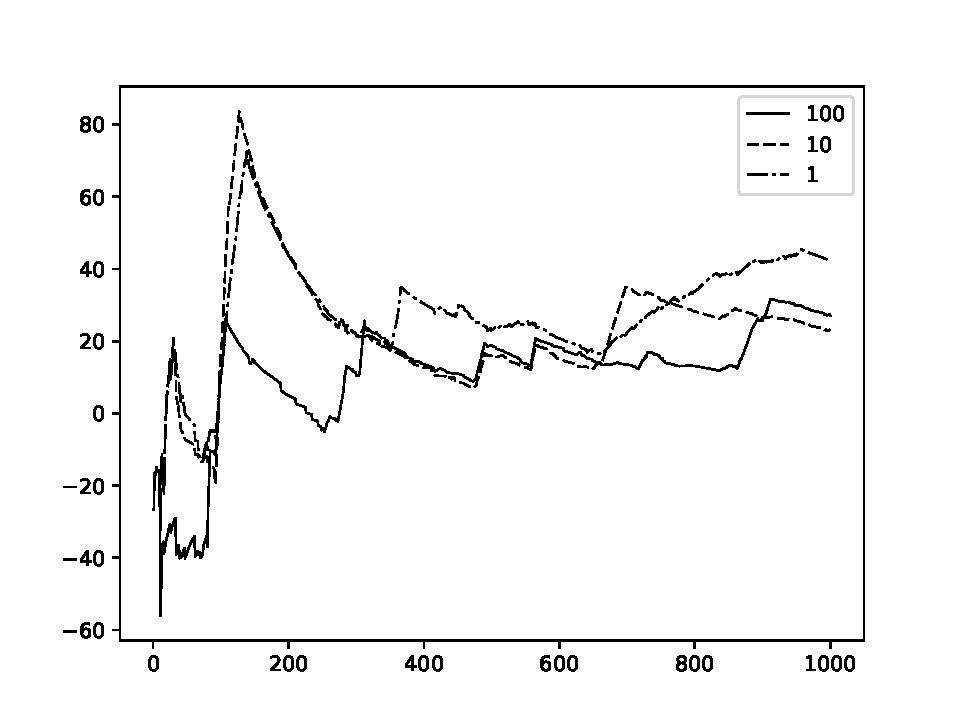
\includegraphics[width=\linewidth]{images/likelihoods-lmbda001.pdf}
    \caption{$\gamma = 0.01$}
    \label{fig:gamma001}
\end{subfigure}
\begin{subfigure}{\linewidth}
    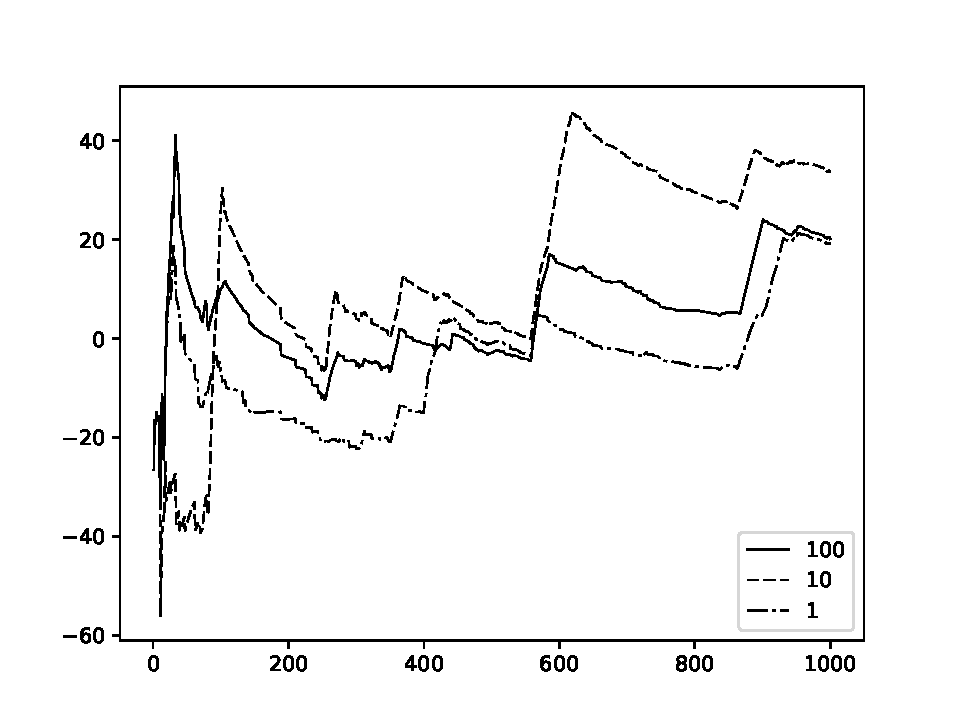
\includegraphics[width=\linewidth]{images/likelihoods-lmbda01.pdf}
    \caption{$\gamma = 0.1$}
    \label{fig:gamma01}
\end{subfigure}
\begin{subfigure}{\linewidth}
    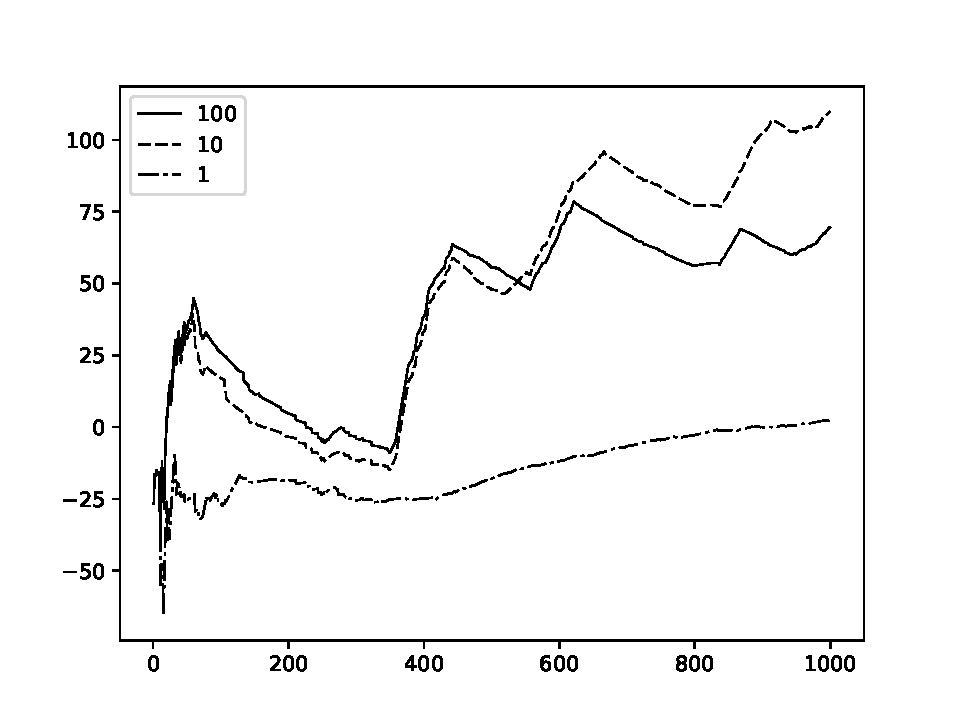
\includegraphics[width=\linewidth]{images/likelihoods-lmbda1.pdf}
    \caption{$\gamma = 1$}
    \label{fig:gamma1}
\end{subfigure}
\caption{Evolution of average log-likelihood of training sentences over parameter updates for minibatches of size 1. Plotted are the performance for $\delta^{(0)} = 1, 10, 100$.}
\label{fig:likelihoods-mb1}
\end{figure}

\begin{figure}{\linewidth}
    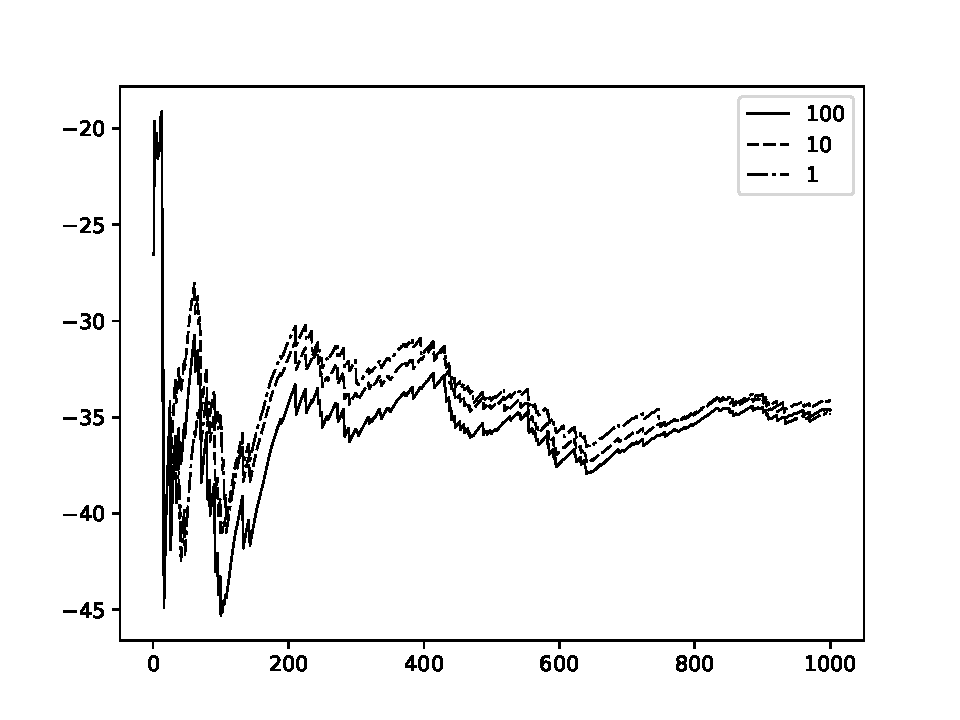
\includegraphics[width=\linewidth]{images/likelihoods-lmbda1-mb10.pdf}
    \caption{Evolution of average log-likelihood of training sentences over parameter updates for minibatches of size 10.}
    \label{fig:likelihoods-mb10}
\end{figure}


\begin{figure}
\begin{subfigure}{\linewidth}
    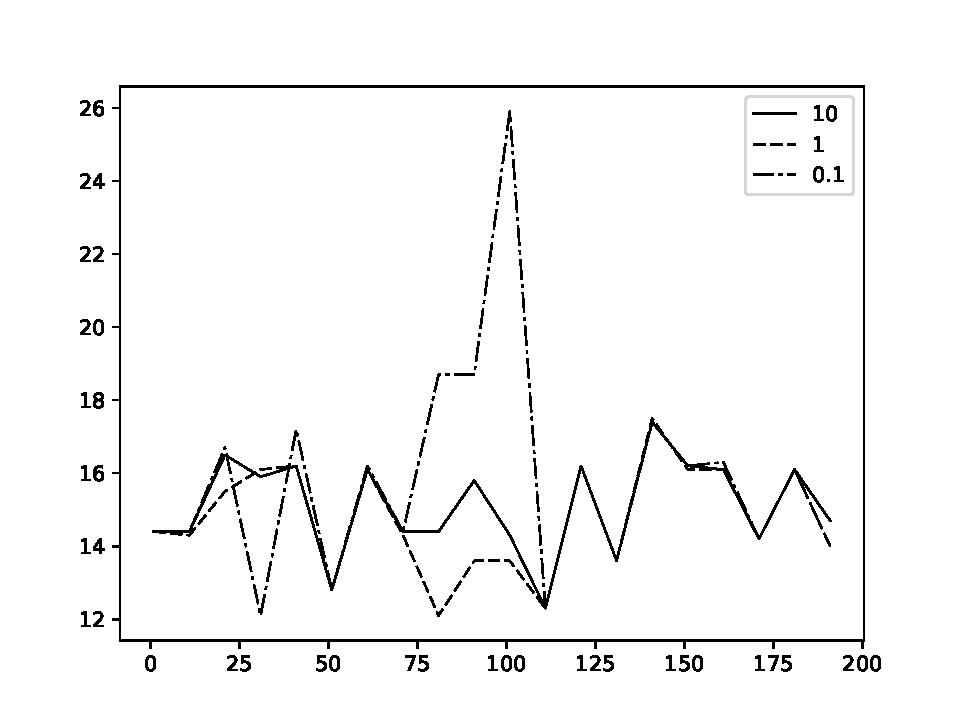
\includegraphics[width=\linewidth]{images/bleu1-mb1.pdf}
    \caption{Minibatch-size 1.}
    \label{fig:bleu1-mb1}
\end{subfigure}
\begin{subfigure}{\linewidth}
    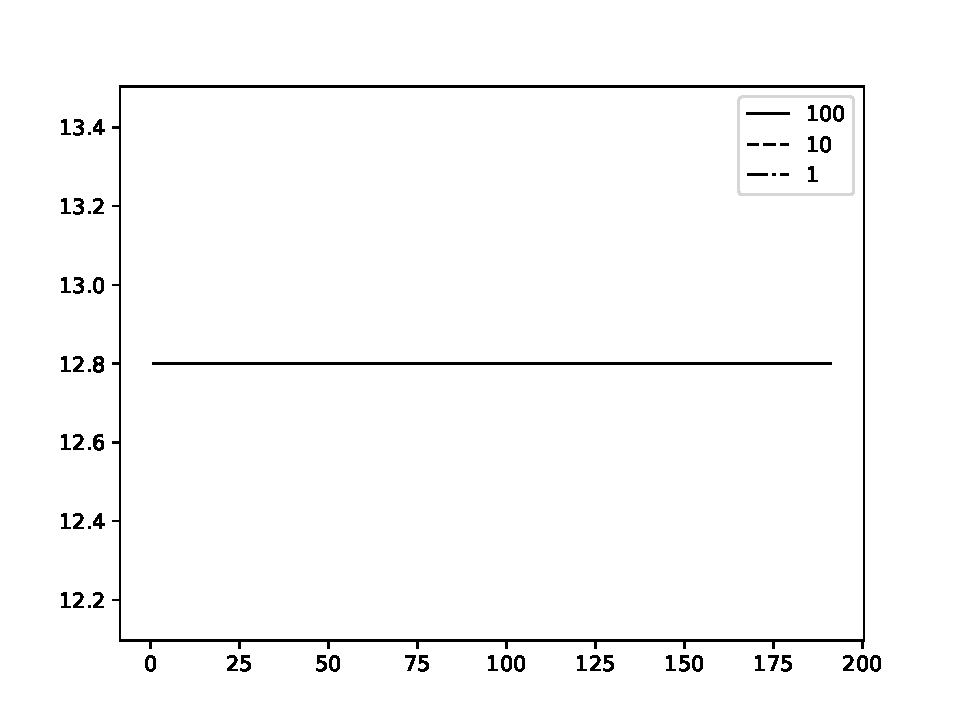
\includegraphics[width=\linewidth]{images/bleu1-mb10.pdf}
    \caption{Minibatch-size 10.}
    \label{fig:bleu1-mb10}
\end{subfigure}
\caption{Evolution of the BLEU1 score. The BLEU score is computed every 10 sentences on a 200-sentence subset of the training-data. For minibatch-size 1 this means 200 parameter-updates were made, and for the minibatch-size 10 only 20. Plotted are the scores for $\delta^{(0)} = 1, 10, 100$. (Note: typo in the legend of plot (a))}
\label{fig:bleu1}
\end{figure}



\end{document}
